\documentclass[11pt]{article}
\usepackage{amsmath,amssymb}
\usepackage{graphicx}
\usepackage{booktabs}
\usepackage{hyperref}
\usepackage[margin=1in]{geometry}
\usepackage{natbib}
\usepackage{multirow}
\usepackage{caption}
\usepackage{enumitem}
\usepackage{tikz}
\usepackage{listings}
\usepackage{xcolor}
\usetikzlibrary{arrows.meta,positioning,shapes.geometric,fit,backgrounds,calc}

\lstset{
  basicstyle=\ttfamily\scriptsize,
  backgroundcolor=\color{gray!8},
  frame=single,
  framerule=0.4pt,
  rulecolor=\color{gray!40},
  breaklines=true,
  columns=fullflexible,
  keepspaces=true,
  aboveskip=6pt,
  belowskip=6pt,
}

% Consistent paragraph spacing
\setlength{\parskip}{0.6em}
\setlength{\parindent}{1em}

\title{Recursive Self-Improvement for Continual Adaptation in Code Generation}

\author{
  Aaditya Nalawade \\
  Department of Computer Science\\
  Stanford University\\
  \texttt{aaditya1@stanford.edu}
  \and
  Chandra Suda \\
  Department of Computer Science\\
  Stanford University\\
  \texttt{csuda@stanford.edu}
  \and
  Ethan Goodhart \\
  Department of Computer Science\\
  Stanford University\\
  \texttt{goodhart@stanford.edu}
}

\date{}

\begin{document}
\maketitle

\begin{abstract}
We present a self-improving code generation agent that combines Self-Distilled Policy Optimization (SDPO) with Retrieval-Augmented Generation (RAG) under a prompt-based routing policy. Given a stream of competitive programming problems and \emph{only} a test-case verifier, the agent autonomously generates solutions, diagnoses failures through recursive feedback cycles, distills successful strategies back into its own parameters, and externalizes reusable lessons into a vector-indexed knowledge store, all without ever requiring golden solutions. On LiveCodeBench, our best configuration improves the solve rate of Qwen2.5-7B-Instruct from 32\% to 38\% (+6\,pp) with 4 recursive attempts per rollout, while test-case accuracy rises from 51.3\% to 55.9\%. Ablations across attempt counts (4, 16, 32), model scales (1.5B vs.\ 7B), and adaptation strategies reveal that (a)~a threshold level of base capability is required for self-improvement to emerge, (b)~SDPO-only consistently outperforms SDPO+RAG at small knowledge-base scales, and (c)~increasing recursive attempts beyond 4 degrades evaluation performance despite improving training-time solution discovery.
\end{abstract}

\section{Introduction}

Deployed language models must continuously acquire new skills without forgetting prior ones, a challenge known as \emph{continual learning}~\citep{kirkpatrick2017forgetting}. Self-Distillation Fine-Tuning (SDFT)~\citep{shenfeld2026sdft} addresses this with a demonstration-conditioned teacher copy that generates on-policy training signals, but it applies parametric updates indiscriminately and relies on externally provided demonstrations.

We propose \textbf{recursive self-improvement}: rather than requiring golden solutions, our agent bootstraps its own improvement using only a test-case verifier that provides rich structured feedback (error traces, failing inputs, execution diagnostics). A model capable of occasionally solving a problem across several attempts can \emph{distill that success back into itself}, progressively expanding the frontier of problems it can reliably solve. To our knowledge, this is the first system where a model improves itself through self-distillation in a fully autonomous loop: it generates and recursively refines solutions, externalizes reusable lessons into a retrievable knowledge store, and directs its own learning through prompt-based tool calls that select adaptation actions. No golden solutions are ever supplied.

Our contributions are:
\begin{itemize}[nosep]
    \item A recursive self-improvement framework requiring only verifier feedback, combining on-policy self-distillation with externalized knowledge under a prompt-based routing policy the model controls itself.
    \item An empirical evaluation on LiveCodeBench with Qwen2.5-7B-Instruct~\citep{qwen2025qwen25}, achieving +6\,pp solve rate through pure self-improvement.
    \item Ablation studies across recursive attempt counts, model scales, and adaptation strategies that reveal critical design constraints for self-improving agents, including a paradoxical finding that more training-time attempts improve solution discovery but degrade evaluation performance.
\end{itemize}

\section{Related Work}

Knowledge distillation~\citep{hinton2015distilling} trains a student to match a teacher; SDFT~\citep{shenfeld2026sdft} makes this on-policy by conditioning the teacher on demonstrations, and SPIN~\citep{chen2024spin} shows self-play can convert weak models into strong ones. Our work eliminates the need for external demonstrations entirely. STaR~\citep{zelikman2022star} bootstraps reasoning by training on correct chain-of-thought traces; we use distillation rather than rejection sampling and add a recursive feedback loop. For memory externalization, MemoryBank~\citep{zhong2024memorybank} augments LLMs with long-term memory, and RAG~\citep{lewis2020rag} augments generation with retrieved documents. We use externalized memory for \emph{lesson consolidation}: storing algorithmic insights from failures for retrieval during future problems, giving the model a non-parametric self-improvement channel alongside parametric weight updates.

\section{Approach}

\subsection{System Architecture}

Our agent consists of four components: a \textbf{student model} (Qwen2.5-7B-Instruct), an \textbf{EMA teacher} (exponential moving average copy), a \textbf{RAG knowledge store} (FAISS-indexed vector database~\citep{johnson2019faiss}), and a \textbf{prompt-based router} (the student model itself, prompted to select adaptation actions). Figure~\ref{fig:architecture} illustrates the full system.

\begin{figure}[t]
\centering
\resizebox{\textwidth}{!}{%
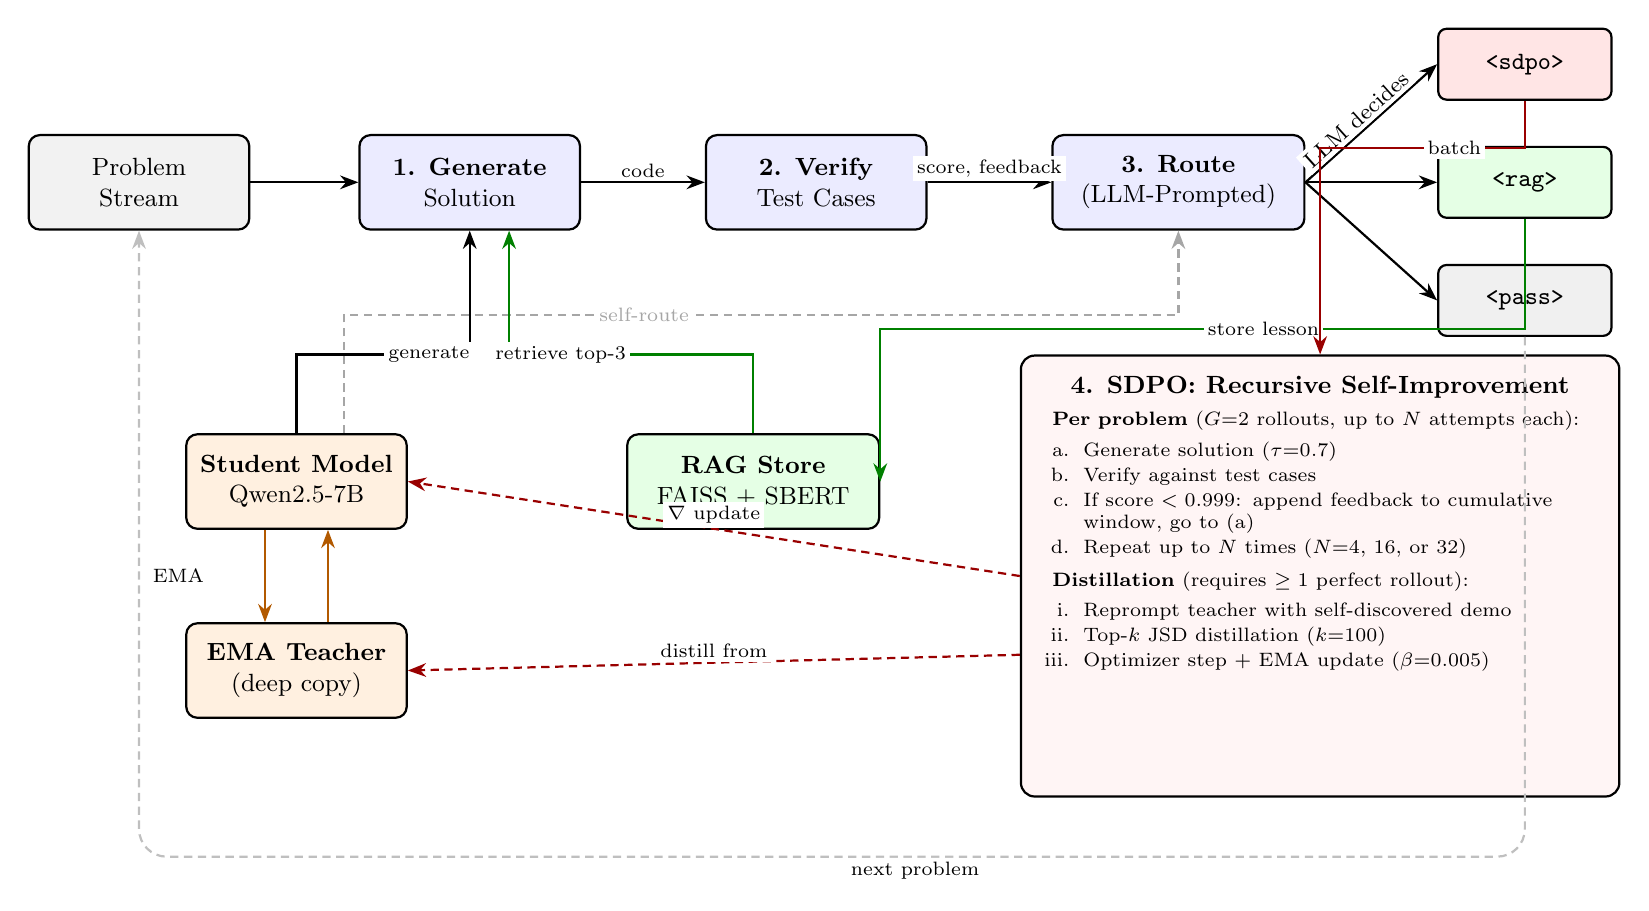
\begin{tikzpicture}[
    >=Stealth,
    every node/.style={font=\small},
    box/.style={draw, rounded corners=4pt, minimum height=1.2cm, minimum width=2.8cm, align=center, line width=0.8pt},
    phase/.style={box, fill=blue!8},
    model/.style={box, fill=orange!12},
    store/.style={box, fill=green!10, minimum width=3.2cm},
    act/.style={draw, rounded corners=3pt, minimum height=0.9cm, minimum width=2.2cm, align=center, line width=0.8pt, font=\small},
    arr/.style={->, line width=0.8pt, >=Stealth},
    darr/.style={->, line width=0.8pt, >=Stealth, densely dashed},
    lbl/.style={font=\scriptsize, fill=white, inner sep=1.5pt},
]

% === TOP ROW: Main pipeline ===
\node[box, fill=gray!10] (problem) at (0, 0) {Problem\\Stream};
\node[phase]             (gen)     at (4.2, 0) {\textbf{1. Generate}\\Solution};
\node[phase]             (ver)     at (8.6, 0) {\textbf{2. Verify}\\Test Cases};
\node[phase, minimum width=3.2cm] (rte) at (13.2, 0) {\textbf{3. Route}\\(LLM-Prompted)};

% === RIGHT COLUMN: Three action boxes ===
\node[act, fill=red!10]   (a_sdpo) at (17.6, 1.5)  {\texttt{<sdpo>}};
\node[act, fill=green!10] (a_rag)  at (17.6, 0)    {\texttt{<rag>}};
\node[act, fill=gray!12]  (a_pass) at (17.6, -1.5) {\texttt{<pass>}};

% === BOTTOM-LEFT: Student + Teacher ===
\node[model] (student) at (2, -3.8) {\textbf{Student Model}\\Qwen2.5-7B};
\node[model] (teacher) at (2, -6.2) {\textbf{EMA Teacher}\\(deep copy)};

% === BOTTOM-CENTER: RAG Store ===
\node[store] (rag) at (7.8, -3.8) {\textbf{RAG Store}\\FAISS + SBERT};

% === BOTTOM-RIGHT: SDPO with Recursive Improvement ===
\node[draw, rounded corners=5pt, fill=red!4, line width=0.8pt,
      minimum width=7.6cm, minimum height=5.6cm] (sdpo_box) at (15.0, -5.0) {};
\node[font=\small\bfseries, anchor=north] at ([yshift=-0.15cm]sdpo_box.north)
      {4. SDPO: Recursive Self-Improvement};

\node[font=\scriptsize, text width=6.8cm, align=left, anchor=north] at ([yshift=-0.6cm]sdpo_box.north) {
    \textbf{Per problem} ($G{=}2$ rollouts, up to $N$ attempts each):\\[3pt]
    \begin{enumerate}[nosep,leftmargin=1.4em,label=\alph*.,itemsep=1pt]
    \item Generate solution ($\tau{=}0.7$)
    \item Verify against test cases
    \item If score $< 0.999$: append feedback to
          cumulative window, go to (a)
    \item Repeat up to $N$ times
          {\scriptsize ($N{=}4$, $16$, or $32$)}
    \end{enumerate}
    \vspace{4pt}
    \textbf{Distillation} (requires $\geq 1$ perfect rollout):\\[3pt]
    \begin{enumerate}[nosep,leftmargin=1.4em,label=\roman*.,itemsep=1pt]
    \item Reprompt teacher with self-discovered demo
    \item Top-$k$ JSD distillation ($k{=}100$)
    \item Optimizer step + EMA update ($\beta{=}0.005$)
    \end{enumerate}
};

% ═══════════════════════════════════
% ARROWS -- Main pipeline
% ═══════════════════════════════════
\draw[arr] (problem) -- (gen);
\draw[arr] (gen)     -- (ver) node[lbl, midway, above] {code};
\draw[arr] (ver)     -- (rte) node[lbl, midway, above] {score, feedback};

% -- Route -> actions (prompt-based) --
\draw[arr] (rte.east) -- (a_sdpo.west) node[lbl, pos=0.45, above, sloped] {\footnotesize LLM decides};
\draw[arr] (rte.east) -- (a_rag.west);
\draw[arr] (rte.east) -- (a_pass.west);

% ═══════════════════════════════════
% ARROWS -- Student / Teacher / RAG
% ═══════════════════════════════════

% Student -> Generate
\draw[arr] (student.north) -- ++(0,1.0) -| (gen.south)
    node[lbl, pos=0.25, right] {generate};

% Student --> Route  (self-routing, dashed)
\draw[darr, gray!70] ([xshift=0.6cm]student.north) -- ++(0,1.5) -| (rte.south)
    node[lbl, pos=0.15, right] {self-route};

% RAG -> Generate  (retrieve)
\draw[arr, green!50!black] (rag.north) -- ++(0,1.0) -| ([xshift=0.5cm]gen.south)
    node[lbl, pos=0.25, left, text=black] {retrieve top-3};

% <rag> -> RAG Store  (store lesson)
\draw[arr, green!50!black] (a_rag.south) -- ++(0,-1.4) -| (rag.east)
    node[lbl, pos=0.25, right, text=black] {store lesson};

% Teacher <-> Student  (EMA)
\draw[arr, orange!70!black] ([xshift=-0.4cm]student.south) -- ([xshift=-0.4cm]teacher.north);
\draw[arr, orange!70!black] ([xshift=0.4cm]teacher.north) -- ([xshift=0.4cm]student.south);
\node[lbl, text=black] at ([xshift=-1.5cm]$(student.south)!0.5!(teacher.north)$) {EMA};

% <sdpo> -> SDPO box
\draw[arr, red!60!black] (a_sdpo.south) -- ++(0,-0.6) -| (sdpo_box.north)
    node[lbl, pos=0.25, right, text=black] {batch};

% SDPO box --> Student  (gradient update)
\draw[darr, red!60!black] (sdpo_box.west) -- (student.east)
    node[lbl, midway, above, text=black] {$\nabla$ update};

% SDPO box --> Teacher  (distill from)
\draw[darr, red!60!black] ([yshift=-1.0cm]sdpo_box.west) -- (teacher.east)
    node[lbl, midway, above, text=black] {distill from};

% -- Loop back (next problem) --
\draw[arr, gray!50, densely dashed, rounded corners=10pt]
    (a_pass.south) -- ++(0,-6.6) -| (problem.south)
    node[lbl, pos=0.22, below, text=black] {next problem};

\end{tikzpicture}%
}
\caption{Architecture of the recursive self-improvement system. For each problem: \textbf{(1)}~the student generates a solution with optional RAG context, \textbf{(2)}~the solution is verified against test cases, \textbf{(3)}~the student-as-router selects an adaptation action via prompt-based reasoning (with rule-based fallback), and \textbf{(4)}~the chosen action executes. The SDPO path triggers recursive self-improvement: $G{=}2$ rollouts each perform up to $N$ sequential attempts with cumulative feedback. Only rollouts achieving $\geq$99.9\% accuracy are used for distillation. No golden solutions are provided at any stage.}
\label{fig:architecture}
\end{figure}

For each problem in the training stream, the agent executes a four-phase loop:

\begin{enumerate}[nosep]
    \item \textbf{Generate}: Build a code prompt from the problem description and test specification. Query the RAG store for relevant knowledge chunks (top-3 by cosine similarity using Sentence-BERT embeddings~\citep{reimers2019sentencebert}). Generate a solution greedily (temperature = 0).
    \item \textbf{Verify}: Execute the solution against test cases in a sandboxed environment. Obtain a score (fraction of tests passed), accuracy, and structured feedback describing which tests failed and why, including error traces and execution diagnostics.
    \item \textbf{Route}: The student model, prompted with the problem summary, score, and feedback, outputs one of three action tags via prompt-based reasoning:
    \begin{itemize}[nosep]
        \item \texttt{<pass>}: Solution is correct or near-correct; no adaptation needed.
        \item \texttt{<rag>}: Partial success with specific, transferable errors. Store a concise lesson.
        \item \texttt{<sdpo>}: Fundamental failure requiring parametric improvement. Queue for self-distillation.
    \end{itemize}
    A rule-based fallback triggers only if the model's output cannot be parsed (score $\geq 0.9 \to$ pass, $0 < \text{score} < 0.9 \to$ rag, score $= 0 \to$ sdpo).
    \item \textbf{Adapt}: Execute the routed action. SDPO problems are batched before executing a gradient step.
\end{enumerate}

\subsection{Self-Distilled Policy Optimization (SDPO)}

When a batch of SDPO-routed problems is collected, we execute the recursive self-improvement and distillation process. This is the core mechanism through which the model improves itself using only verifier feedback.

\paragraph{Phase 1: Recursive rollout generation.} For each problem, we generate $G = 2$ independent rollouts. Each rollout proceeds as a recursive self-improvement loop for up to $N$ sequential attempts (where $N \in \{4, 16, 32\}$ across our experimental configurations):

\begin{enumerate}[nosep]
    \item \textbf{Attempt 1}: Generate a solution from the original prompt (temperature $\tau = 0.7$).
    \item \textbf{Verify}: Execute against the test suite. If score $\geq 0.999$ (near-perfect), stop; this rollout has succeeded.
    \item \textbf{Feedback accumulation}: Append the structured failure feedback to a cumulative \emph{feedback window}, a growing context of all prior failed attempts and their error descriptions.
    \item \textbf{Re-attempt}: Re-prompt the model with the original problem plus the full feedback window, explicitly instructing it to analyze prior failures and generate a fundamentally different solution.
    \item Repeat steps 2--4 until success or $N$ attempts exhausted.
\end{enumerate}

The feedback window template explicitly instructs: ``\emph{Carefully analyze each error above, understand WHY the previous approach failed, then choose a DIFFERENT algorithm or fix the root cause. Do NOT repeat the same logic that already failed.}''

Only rollouts achieving $\geq$99.9\% test-case accuracy proceed to distillation. This ensures the teacher is always conditioned on solutions the model \emph{proved correct through its own recursive refinement}.

\paragraph{Phase 2: Reprompted teacher distillation.} For each problem with at least one successful rollout, we construct an enriched teacher prompt containing (a)~the original problem, (b)~the self-discovered correct solution, and (c)~feedback from the initial failed attempt. The EMA teacher performs a forward pass on this reprompted input with no gradients, extracting top-$k$ log-probabilities ($k = 100$) at each response position. The student performs a forward pass on the \emph{original} prompt (without demonstrations) and gathers its log-probabilities at the teacher's top-$k$ indices. We compute Jensen-Shannon Divergence ($\alpha = 0.5$):
\begin{equation}
    \mathcal{L}_{\text{JSD}} = (1 - \alpha) \, \text{KL}(p_s \| m) + \alpha \, \text{KL}(p_t \| m), \quad m = (1-\alpha) \, p_s + \alpha \, p_t
\end{equation}
where $p_t$ and $p_s$ are the teacher and student top-$k$ distributions. A tail probability bucket ($\log(1 - \sum_i p_i)$) accounts for the remaining vocabulary mass. No separate reference model KL penalty is used ($\beta_{\text{ref}} = 0$), eliminating the need for a frozen reference copy and saving ${\sim}$14\,GB VRAM.

\paragraph{Phase 3: Optimizer step and EMA update.} Gradients are scaled by $1/N_{\text{rollouts}}$, clipped ($\|\nabla\|_{\max} = 1.0$), and applied via 8-bit AdamW~\citep{loshchilov2019adamw}. The teacher is then updated: $\theta_t \leftarrow (1 - \beta)\theta_t + \beta\theta_s$ with $\beta = 0.005$.

The teacher has an \emph{informational advantage}: it sees a correct solution the model discovered through recursive self-improvement, so its predictions encode knowledge the student currently lacks. Distilling from this enriched teacher teaches the student to reach correct solutions more directly, without recursive refinement at inference time.

\subsection{RAG Knowledge Store}

When the router selects \texttt{<rag>}, the model generates a concise lesson (2--3 sentences, focusing on the \emph{type} of mistake rather than problem-specific code) along with a truncated problem summary, and stores the combined chunk in a FAISS \texttt{IndexFlatIP} index with Sentence-BERT (\texttt{all-MiniLM-L6-v2}) embeddings~\citep{reimers2019sentencebert}. Each stored chunk contains both the problem context and the extracted lesson, enabling retrieval by problem similarity. During generation, the top-3 most similar chunks are retrieved and prepended as system context, giving the model a non-parametric self-improvement channel.

\subsection{Data}
\label{sec:data}

We use LiveCodeBench~\citep{jain2024livecodebench}, a contamination-free competitive programming benchmark with 924 problems sourced from Codeforces, LeetCode, and AtCoder after model training cutoff dates. Problems span difficulty levels from easy to extremely hard. We split the dataset 70/30: approximately 647 problems for training and 277 for testing. At evaluation time, we subsample 50 test problems for tractable compute.

LiveCodeBench is substantially harder than standard benchmarks: GPT-4 achieves ${\sim}$55\% pass rate versus ${>}$85\% on HumanEval. Our Qwen2.5-7B baseline achieves 32\% solve rate, consistent with 7B-class models on competitive programming.

\subsection{Evaluation Method}

We evaluate five configurations:
\begin{enumerate}[nosep]
    \item \textbf{Baseline 7B}: Qwen2.5-7B-Instruct, no training, no RAG.
    \item \textbf{Model + SDPO}: SDPO-trained 7B model without RAG at inference.
    \item \textbf{Model + RAG + SDPO}: Full system with both SDPO training and RAG retrieval.
    \item \textbf{Baseline 1.5B}: Qwen2.5-1.5B-Instruct, no training.
    \item \textbf{1.5B + SDPO/RAG}: Same pipeline applied to the 1.5B model.
\end{enumerate}

We report \textbf{test-case accuracy} (fraction of individual test cases passed, averaged over problems) and \textbf{solve rate} (fraction of problems where all test cases pass). Evaluation uses greedy decoding (temperature = 0). Checkpoints are saved every 50 training problems.

\subsection{Experimental Details}

All experiments run on NVIDIA A100-80GB GPUs via Modal cloud compute. The model uses BFloat16 precision with gradient checkpointing for memory efficiency.

\begin{table}[h]
\centering
\begin{tabular}{lc}
\toprule
\textbf{Hyperparameter} & \textbf{Value} \\
\midrule
Base model & Qwen2.5-7B-Instruct \\
Learning rate & $2 \times 10^{-6}$ \\
Optimizer & 8-bit AdamW \\
EMA rate ($\beta$) & 0.005 \\
Rollouts per problem ($G$) & 2 \\
Sequential attempts per rollout ($N$) & 4 / 16 / 32 \\
Sampling temperature & 0.7 \\
Distillation top-$k$ & 100 \\
JSD mixture ($\alpha$) & 0.5 \\
Success threshold ($\theta$) & 0.999 \\
Reference KL ($\beta_{\text{ref}}$) & 0.0 (disabled) \\
Max gradient norm & 1.0 \\
RAG top-$k$ retrieval & 3 \\
RAG embedding model & all-MiniLM-L6-v2 \\
\bottomrule
\end{tabular}
\caption{Hyperparameter configuration.}
\label{tab:hyperparams}
\end{table}

We conduct four training runs: three on the 7B model with 4, 16, and 32 sequential attempts per rollout, and one on the 1.5B model with 4 attempts. Each 7B run processes up to 250 training problems with checkpoints at steps 50, 100, 150, 200, and 250.

\subsection{Results}

\paragraph{Main results.} Table~\ref{tab:main} presents the best checkpoint results for each configuration. SDPO-only with 4 attempts achieves the strongest performance at checkpoint 200: 55.9\% test-case accuracy and 38\% solve rate (19/50), a +6\,pp gain over the 7B baseline. This improvement is achieved through pure self-improvement, without ever being shown a golden solution. The 1.5B model not only fails to improve but actively \emph{degrades} under the same pipeline, confirming the capability threshold for self-improvement.

\begin{table}[h]
\centering
\begin{tabular}{lccc}
\toprule
\textbf{Configuration} & \textbf{Test-Case Acc} & \textbf{Solve Rate} & \textbf{Correct} \\
\midrule
Baseline (Qwen 7B) & 0.5130 & 0.3200 & 16/50 \\
\midrule
\multicolumn{4}{l}{\textit{7B, v1 (4 attempts per rollout)}} \\
\quad Model + SDPO & \textbf{0.5595} & \textbf{0.3800} & \textbf{19/50} \\
\quad Model + RAG + SDPO & 0.5200 & 0.3400 & 17/50 \\
\midrule
\multicolumn{4}{l}{\textit{7B, v2 (16 attempts per rollout)}} \\
\quad Model + SDPO & 0.5545 & 0.3000 & 15/50 \\
\quad Model + RAG + SDPO & 0.4760 & 0.3200 & 16/50 \\
\midrule
\multicolumn{4}{l}{\textit{7B, v3 (32 attempts per rollout)}} \\
\quad Model + SDPO & 0.5305 & 0.3000 & 15/50 \\
\quad Model + RAG + SDPO & 0.4715 & 0.2800 & 14/50 \\
\midrule
Baseline (Qwen 1.5B) & 0.1400 & 0.1400 & 7/50 \\
\quad 1.5B + SDPO & 0.0800 & 0.0800 & 4/50 \\
\quad 1.5B + RAG + SDPO & 0.1000 & 0.1000 & 5/50 \\
\quad 1.5B + RAG only & 0.1200 & 0.1200 & 6/50 \\
\bottomrule
\end{tabular}
\caption{Performance on 50 test problems (best checkpoint per configuration). The 7B SDPO-only with 4 attempts achieves the best result. The 1.5B model degrades after training, establishing a capability threshold.}
\label{tab:main}
\end{table}

\paragraph{Training dynamics.} Table~\ref{tab:checkpoints} shows how performance evolves across training checkpoints for the best configuration (v1, 4 attempts). SDPO-only shows steady gains, peaking at step 200 with 38\% solve rate (+6\,pp over baseline). Performance slightly regresses at step 250, suggesting the onset of overfitting. RAG+SDPO consistently underperforms SDPO-only at every checkpoint.

\begin{table}[h]
\centering
\begin{tabular}{ccccc}
\toprule
\textbf{Step} & \textbf{SDPO Acc} & \textbf{SDPO Solve} & \textbf{RAG+SDPO Acc} & \textbf{RAG+SDPO Solve} \\
\midrule
50 & 54.4\% & 32\% & 50.8\% & 32\% \\
100 & \textbf{56.5\%} & 36\% & 53.6\% & 34\% \\
150 & 54.9\% & 36\% & \textbf{53.9\%} & 34\% \\
200 & 55.9\% & \textbf{38\%} & 51.8\% & 34\% \\
250 & 52.9\% & 36\% & 54.9\% & 32\% \\
\bottomrule
\end{tabular}
\caption{Training checkpoint progression for v1 (4 recursive attempts). Baseline: 51.3\% accuracy, 32\% solve rate.}
\label{tab:checkpoints}
\end{table}

\paragraph{Effect of recursive attempt count.} Increasing recursive attempts from 4 to 16 or 32 does \emph{not} improve evaluation results and in fact degrades them (Table~\ref{tab:main}). With 16 attempts, SDPO solve rate drops to 30\%; with 32 attempts, RAG+SDPO falls to 28\%. We hypothesize that with more recursive attempts, the model learns to hardcode edge-case fixes rather than developing genuine algorithmic understanding. The cumulative feedback window becomes increasingly long and specific, encouraging pattern-matched special cases rather than general solutions.

\paragraph{The attempt-count paradox.} While more attempts \emph{degrade} evaluation performance, they substantially \emph{improve} training-time solution discovery. Table~\ref{tab:perfects} shows this relationship. The percentage of perfect solutions discovered through recursive refinement (attempt $> 1$) increases dramatically with more attempts: 62\% at $N{=}4$, 80\% at $N{=}16$, and 84\% at $N{=}32$. Yet this improved discovery does not translate to better generalization, revealing a critical design tension: more refinement attempts help the model find correct solutions for training, but the solutions found through extensive trial-and-error may be lower quality (overfitted to specific edge cases) and thus produce worse distillation targets.

\begin{table}[h]
\centering
\begin{tabular}{lcccccc}
\toprule
\textbf{Config} & \textbf{Perfects} & \textbf{Att.\ 1} & \textbf{Att.\ $>$1} & \textbf{\% from Att.\ $>$1} & \textbf{Eval Solve Rate} \\
\midrule
v1 ($N{=}4$)  & 106 & 40 & 66 & 62\% & \textbf{38\%} \\
v2 ($N{=}16$) & 54  & 11 & 43 & 80\% & 30\% \\
v3 ($N{=}32$) & 67  & 11 & 56 & 84\% & 30\% \\
\bottomrule
\end{tabular}
\caption{The attempt-count paradox: more recursive attempts improve training-time solution discovery but degrade evaluation performance. ``Perfects'' counts rollouts achieving $\geq$99.9\% accuracy. Despite 84\% of v3 perfects coming from recursive refinement, v3 evaluation solve rate (30\%) is worse than v1 (38\%).}
\label{tab:perfects}
\end{table}

\paragraph{SDPO-only vs.\ SDPO+RAG.} Across all configurations and checkpoints, SDPO-only consistently outperforms SDPO+RAG. At the best checkpoint (v1, step 200): SDPO achieves 55.9\% accuracy vs.\ 52.0\% for RAG+SDPO, and 38\% vs.\ 34\% solve rate. We attribute this to the small scale of the RAG knowledge base: with only $\sim$20--30 stored chunks by step 200, retrieval introduces more noise than signal.

\paragraph{1.5B model ablation.} The Qwen2.5-1.5B-Instruct model not only fails to improve but actually \emph{degrades} under the same pipeline (Table~\ref{tab:main}, bottom). The 1.5B baseline achieves 14\% solve rate (7/50); after SDPO training, this drops to 8\% (4/50). The 1.5B model cannot generate sufficiently diverse and correct rollouts to provide demonstrations for the teacher, and the distillation from low-quality demonstrations actively harms performance. This establishes a clear \emph{capability threshold} below which recursive self-improvement is not viable.

\section{Analysis}

\paragraph{Verifier-only self-improvement.} A critical property of our system is that no golden solutions are ever provided. The entire pipeline operates with only a test-case verifier providing rich structured feedback (error traces, failing inputs, execution diagnostics). The model uses this signal to recursively refine its approach. When it discovers a correct solution, it distills that self-discovered knowledge into its weights. This is genuine recursive self-improvement: the model is both the learner and the source of training signal, with the verifier serving only as an objective function.

\paragraph{Prompt-based routing.} The routing decision is made by the model itself through prompting, not by hard-coded rules. The model receives the problem summary, score, and failure feedback, then reasons about the appropriate learning action. This means the model participates in directing its own learning process, a form of meta-learning where the agent autonomously decides when to update weights versus when to store knowledge externally. The rule-based fallback activates only when the model's routing output cannot be parsed.

\paragraph{Training dynamics: routing breakdown.} Table~\ref{tab:routing} shows the routing decisions across training runs. The v1 configuration (500 problems processed) routes 52\% of problems to SDPO, 14\% to RAG, and 34\% to PASS. The high PASS rate (34\%) reflects problems the model can already solve correctly on first attempt, consistent with its 32\% baseline solve rate.

\begin{table}[h]
\centering
\begin{tabular}{lccccccc}
\toprule
\textbf{Config} & \textbf{Problems} & \textbf{SDPO} & \textbf{RAG} & \textbf{PASS} & \textbf{Perfects} & \textbf{From Att.\ $>1$} \\
\midrule
v1 ($N{=}4$)  & 500 & 261 & 69 & 170 & 106 & 66 (62\%) \\
v2 ($N{=}16$) & 250 & 81  & 56 & 113 & 54  & 43 (80\%) \\
v3 ($N{=}32$) & 200 & 63  & 39 & 98  & 67  & 56 (84\%) \\
\bottomrule
\end{tabular}
\caption{Routing breakdown and solution discovery across training configurations.}
\label{tab:routing}
\end{table}

\paragraph{RAG knowledge quality.} To understand why RAG did not help quantitatively, we examine what the model chose to store. Figure~\ref{fig:ragchunk} shows a representative chunk.

\begin{figure}[h]
\centering
\begin{minipage}{0.92\textwidth}
\begin{lstlisting}
Problem summary: You are given a string s consisting of only
lowercase English letters. In one operation, you can do the
following: Select any non-empty substring of s, possibly the
entire string, then replace each one of its characters with
the previous character of the En...

Lesson: The solution likely attempted to process the entire
string in a single pass without properly managing the time
complexity, leading to a Time Limit Exceeded error. In similar
problems, be cautious of operations that require processing
substrings repeatedly or in a nested manner, as they can quickly
become inefficient, especially with large inputs.
\end{lstlisting}
\end{minipage}
\caption{Example RAG chunk from the externalized knowledge store. Each chunk contains a truncated problem summary and a model-generated lesson focusing on the \emph{type} of mistake. The model autonomously decides when to store such lessons via the prompt-based routing policy.}
\label{fig:ragchunk}
\end{figure}

The stored chunks capture genuine algorithmic insights (e.g., ``carefully consider overlapping intervals,'' ``ensure the algorithm correctly identifies the longest valid substring''). However, they are too sparse ($\sim$20--30 chunks by step 200) to reliably match dissimilar test problems, introducing noise into the generation context rather than helping.

\paragraph{Compute considerations.} Each training run processes 200--250 problems on a single A100-80GB over approximately 12 hours. We conducted 4 complete training runs, representing a manageable compute budget for an academic setting. The SDPO update is the bottleneck: each batch requires $G \times N$ potential generation passes plus teacher and student forward passes for distillation.

\paragraph{Failure analysis.} With 16 and 32 recursive attempts, we observe performance degradation despite improved solution discovery. Inspection of training logs reveals that with more attempts, the model increasingly generates solutions that pass test cases by hardcoding expected outputs for specific inputs rather than fixing the underlying algorithmic logic. The recursive feedback loop amplifies this pattern. Addressing this will require richer feedback mechanisms, potentially incorporating chain-of-thought reasoning about \emph{why} a solution is wrong rather than simply reporting which tests fail.

\section{Conclusion}

We presented a recursive self-improvement framework for code generation that combines self-distilled policy optimization with externalized knowledge storage under a prompt-based routing policy. The entire self-improvement process requires only a verifier providing rich structured feedback; no golden solutions, human demonstrations, or external teachers are needed. The model generates solutions, recursively refines them, discovers correct approaches through trial-and-error, and distills this self-discovered knowledge into its own parameters.

Our experiments on LiveCodeBench demonstrate +6\,pp solve rate improvement through pure self-improvement, but reveal important constraints: (a)~more recursive attempts paradoxically improve training-time solution discovery while degrading evaluation performance, (b)~externalized memory via RAG introduces noise at small scale, and (c)~a minimum base capability is required for the self-improvement loop to function (the 1.5B model actively degrades). These findings highlight both the promise and the challenges of recursive self-improvement: the model can genuinely teach itself, but the quality of self-generated training signal is as important as its quantity.

\section*{Team Contributions}

\textbf{Aaditya Nalawade}: Led the SDPO implementation including the self-distillation update, top-$k$ KL divergence loss computation, reprompted teacher design, and EMA teacher management. Ran training experiments on Modal A100 infrastructure.

\textbf{Chandra Suda}: Implemented the RAG knowledge store, prompt-based routing policy, and verification pipeline. Designed and ran the evaluation framework with ablation configurations across checkpoints.

\textbf{Ethan Goodhart}: Built the main training loop, model architecture, and generation infrastructure. Coordinated experimental design across attempt-count and model-scale ablations. Led analysis and paper writing.

\bibliographystyle{unsrt}
\bibliography{references}

\end{document}
